\documentclass[border=4pt]{standalone}
\usepackage{fontspec}
\usepackage{amsmath}
\usepackage{unicode-math}
\setmainfont{Latin Modern Roman}
\setmathfont{Latin Modern Math}
\usepackage{pgfplots}
\usepackage{pgfplotstable}
\pgfplotsset{compat=1.18}
\usepackage{tkz-euclide}
\usetikzlibrary{arrows.meta,calc,angles,quotes,patterns,3d,backgrounds}
\definecolor{ink}{HTML}{123428}
\definecolor{asy}{HTML}{475569}
\definecolor{mint}{HTML}{86e0bd}
\tikzset{asym/.style={asy, line width=0.9pt, dash pattern=on 5pt off 3.5pt},
         guide/.style={gray!70, line width=0.6pt, densely dotted},
         dot/.style={circle, inner sep=0pt, minimum size=5pt, draw=white, line width=0.5pt},
         odot/.style={circle, inner sep=0pt, minimum size=5.5pt, fill=white, line width=1pt},
         lab/.style={font=\footnotesize, inner sep=1.5pt, text=ink}}
\begin{document}
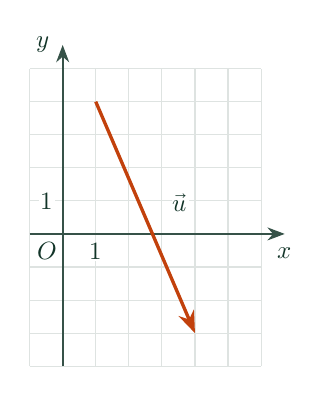
\begin{tikzpicture}
\draw[ink!14, line width=0.4pt] (0.000,0.000) -- (0.000,3.780);
\draw[ink!14, line width=0.4pt] (0.420,0.000) -- (0.420,3.780);
\draw[ink!14, line width=0.4pt] (0.840,0.000) -- (0.840,3.780);
\draw[ink!14, line width=0.4pt] (1.260,0.000) -- (1.260,3.780);
\draw[ink!14, line width=0.4pt] (1.680,0.000) -- (1.680,3.780);
\draw[ink!14, line width=0.4pt] (2.100,0.000) -- (2.100,3.780);
\draw[ink!14, line width=0.4pt] (2.520,0.000) -- (2.520,3.780);
\draw[ink!14, line width=0.4pt] (2.940,0.000) -- (2.940,3.780);
\draw[ink!14, line width=0.4pt] (0.000,0.000) -- (2.940,0.000);
\draw[ink!14, line width=0.4pt] (0.000,0.420) -- (2.940,0.420);
\draw[ink!14, line width=0.4pt] (0.000,0.840) -- (2.940,0.840);
\draw[ink!14, line width=0.4pt] (0.000,1.260) -- (2.940,1.260);
\draw[ink!14, line width=0.4pt] (0.000,1.680) -- (2.940,1.680);
\draw[ink!14, line width=0.4pt] (0.000,2.100) -- (2.940,2.100);
\draw[ink!14, line width=0.4pt] (0.000,2.520) -- (2.940,2.520);
\draw[ink!14, line width=0.4pt] (0.000,2.940) -- (2.940,2.940);
\draw[ink!14, line width=0.4pt] (0.000,3.360) -- (2.940,3.360);
\draw[ink!14, line width=0.4pt] (0.000,3.780) -- (2.940,3.780);
\draw[ink!85, line width=0.7pt, -{Stealth[length=2.2mm]}] (0.000,1.680) -- (3.240,1.680);
\draw[ink!85, line width=0.7pt, -{Stealth[length=2.2mm]}] (0.420,0.000) -- (0.420,4.080);
\node[font=\small, text=ink] at (3.240,1.430) {$x$};
\node[font=\small, text=ink] at (0.170,4.080) {$y$};
\draw[color={rgb,255:red,194;green,65;blue,12}, line width=1.2pt, -{Stealth[length=2.8mm]}] (0.840,3.360) -- (2.100,0.420);
\node[font=\small, text=ink, inner sep=0.5pt, fill=white] at (1.911,2.079) {$\vec u$};
\node[font=\small, text=ink, inner sep=0.5pt, fill=white] at (0.220,1.460) {$O$};
\node[font=\small, text=ink, inner sep=0.5pt, fill=white] at (0.840,1.460) {$1$};
\node[font=\small, text=ink, inner sep=0.5pt, fill=white] at (0.220,2.100) {$1$};
\end{tikzpicture}
\end{document}
